\chapter{Minecraft}
To understand how and why the video game Minecraft is expected to be an interesting simulation environment for artificial general intelligence, necessary background information, about what makes Minecraft different from many other games, has to be given first. To furthermore work with it, the basic elements of the game's architecture have to be described. This chapter provides a roundup of Minecraft's history and a brief explanation of the basic game mechanics. They are followed by an overview of Minecraft uses, that exceed the original game's purpose as well as an explanation, of why Minecraft is suitable as a simulation environment. Eventually, related software projects, that have been used for this thesis, are introduced and described.

    \section{Overview}
The story of Minecraft has many interesting sides, but first and foremost it is a story of immense, unexpected success. To give an overview of it, this section delivers insights into it's main ideas, as well as a general look at the developer's practices. Moreover, the game's reception is considered, as it is unusually strong. They are based on \emph{Minecraft, beyond construction and survival}~\cite{Duncan:2011:MBC:2207096.2207097}.
    
        \subsection{Main Ideas}
When Markus (``Notch'') Persson built and released the first public version of Minecraft, it soon became clear that his creation resonated with many people. The simple concept of a world entirely build out of standard sized building blocks, which the player can create, destroy and relocate one-by-one, enabled many gamers to employ their creativity, explore the Minecraft world and test out it's possibilities and boundaries.

Looking at the game for the first time, it is impossible to oversee the primitive appearance of it`s graphics engine. Everything in the game is made out of blocks. May it be the leaves of a tree, dirt, people or the clouds. Even the sun does not appear round, but as a cubic object. One can assume, that the obvious connotation to Lego(TM) is more than a coincidence, as it immediately gives the player a clue, about what kind of possibilities for building and creating the game might deliver.

Another interesting aspect about Minecraft is the procedural semantics the game world is generated with. Trees in Minecraft, for example, may share a similar structure that consists of a trunk and leave-covered branches spreading out fractally, but the particular characteristics of each tree are generated randomly. This makes a Minecraft world somewhat more realistic than those of many other videogames.

Minecraft strives to be the opposite of a game with a strict game-flow. Instead, it enables the player's creativity and joy of creation.

        \subsection{Development Process}
The development process of Minecraft is very different from those of most other well-known games. Instead of building the game over months or years to finally release a (more or less) finished version to the public, Minecraft is being designed iteratively. In fact, Persson released the first version only a week after he started working on the game. Ever since, new features have been added and new versions of the game have been released frequently. Another defining aspect of Mojang's approach towards the development of Minecraft is the involvement of the game's players. Since the earliest stages, future plans have been discussed openly and many times the players' voices have been heard. Persson himself locates his approach in the field of agile software development.

        \subsection{Reception}
The game has attracted great attention ever since its first release in 2009. Since copies of the game could be obtained commercially for the first time, different versions of the it sold more than 26 million times---with the PC version priced at about 20 Euros, for example. It should be noted, that Minecraft's development studio Mojang is a so called ``indie game developer'', that is not associated with any classical game publisher, but distributes copies of their game exclusively via their own website.

Minecraft can certainly be called a world wide phenomenon. The games developers received a number of prizes for their creation - not to mention the millions of dollars that have been earned in Minecraft sales. With its huge success, Minecraft has proven clearly that it compelled to many players.

Unlike any other game, Minecraft fosters the creativity of its players. Bringing the construction component to one extreme after the other, well publicised creations include a life-size model of the USS Enterprise-D as well as a fully functional arithmetic unit. Videos of roller coaster rides through complex constructions increasingly show characteristics of an art form themselves---regarding to the amount of views on youtube, not less than other, well established formats.

    \section{Game Mechanics}
Now knowing about the game's background, in this section we will continue with descriptions of the basic concepts of the game, that regards to our AI interface. 

Before a new Minecraft game begins, it procedurally generates a three-dimensional world. The player is then dropped to a spawn point and is now facing a scenario with a minimal game interface, lacking any kind of instruction or advise about what to do next. Soon, the procedural generated world drives most players to explore the highest mountains and deepest caverns. As the player collects resources and crafts items, harder to reach resources and more complex to craft items  become available.~\cite{Duncan:2011:MBC:2207096.2207097}

Although the game can be downloaded and played as a single packet of software, many scenarios of playing the game consist of running a Minecraft server software, as well as one copy of the client software for each player. It is possible to mimic the official client by implementing the reverse-engineered client-server-protocol and therefore build artificial players that way.

The structure of Minecraft worlds and the client-server-protocol are described in the following. The descriptions are based on the regarding articles of the \emph{Minecraft Wiki}~\cite{mcwiki}.

    \subsection{Minecraft Worlds}

\begin{wrapfigure}{r}{0.3\textwidth}
  \begin{center}
    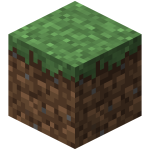
\includegraphics[width=0.15\textwidth]{graphics/block}
  \end{center}
  \caption{A~"Grass"~Block~\cite{image_mob}}
  \label{mc_block}
\end{wrapfigure}

The most important concept in Minecraft is the block~(see figure ~\ref{mc_block}). A block is a cube which sides are, compared to the player, roughly one meter long. Every Minecraft worlds is built up entirely out of them, so the worlds can be thought of as a three dimensional spaces filled with voxels.~\cite{baloghcodemetropolis} There are different types (materials) of blocks and they share their single size, which converts to the basic distance unit of Minecraft.

A chunk~(see figure ~\ref{mc_chunk}) is a segment of the Minecraft world that is 16 blocks long, 16 blocks wide and 256 blocks high (or deep) and therefore consists of up to 65,536 blocks.~\cite{mcwiki_chunks}

\begin{wrapfigure}{r}{0.15\textwidth}
  \begin{center}
    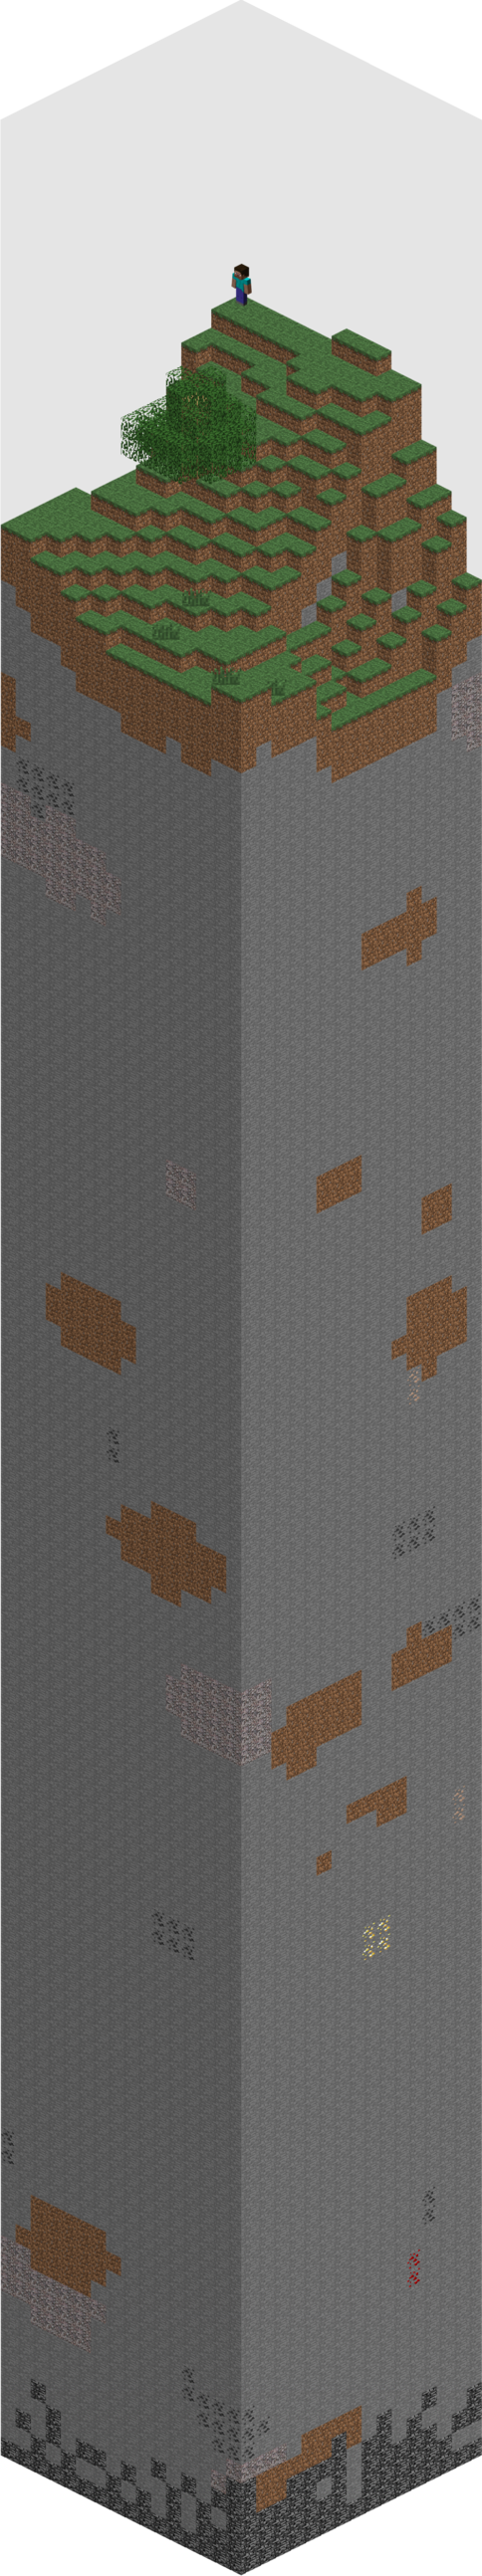
\includegraphics[width=0.16\textwidth]{graphics/chunk}
  \end{center}
  \caption{A~Chunk~\cite{image_mob}}
  \label{mc_chunk}
\end{wrapfigure} 

"The player"~(see figure ~\ref{mc_player}) is what the playable game-character in Minecraft is called. It is usually displayed humanoid.
Also, a Minecraft world has a day-night-cycle with 24 Minecraft hours converting to 14 minutes by default

\begin{wrapfigure}{l}{0.3\textwidth}
  \begin{center}
    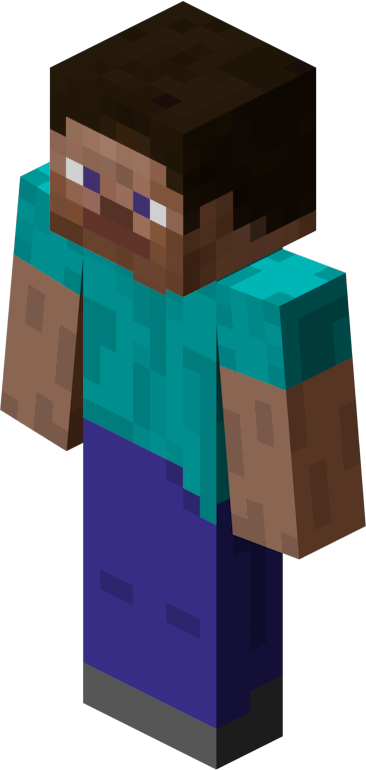
\includegraphics[width=0.08\textwidth]{graphics/player}
  \end{center}
  \caption{"The~Player"~\cite{image_mob}}
  \label{mc_player}
\end{wrapfigure} 

The game itself has no predefined goals. Players can walk around, discover the generated world (see figure \ref{mc_mechanics} 1) and collect resources by ``destroying'' blocks, with the generated resources equaling the block type. They can combine different resources to ``craft'' items. For example, a player can destroy the blocks that represent a tree~(see figure \ref{mc_mechanics} 2). The gained ``wood'' resource could then be used to craft a wooden pickaxe~(see figure \ref{mc_mechanics} 3), which could then be used to dig into the ground more effectively~(see figure \ref{mc_mechanics} 4) to ``mine'' more rare resources, like iron or gold.

There exist different game modes. The original "survival" mode adds monsters that attack the player at night. What solutions to survive the player comes up with (eg. building shelter or fighting the monsters) is left up to him or her.

In "creative" mode, the player is not being attacked by monsters, has the ability to fly and instant access to unlimited resources.

The mode of a Minecraft world does not effect the functionality of this project.

\begin{figure}[h]
  \centering
    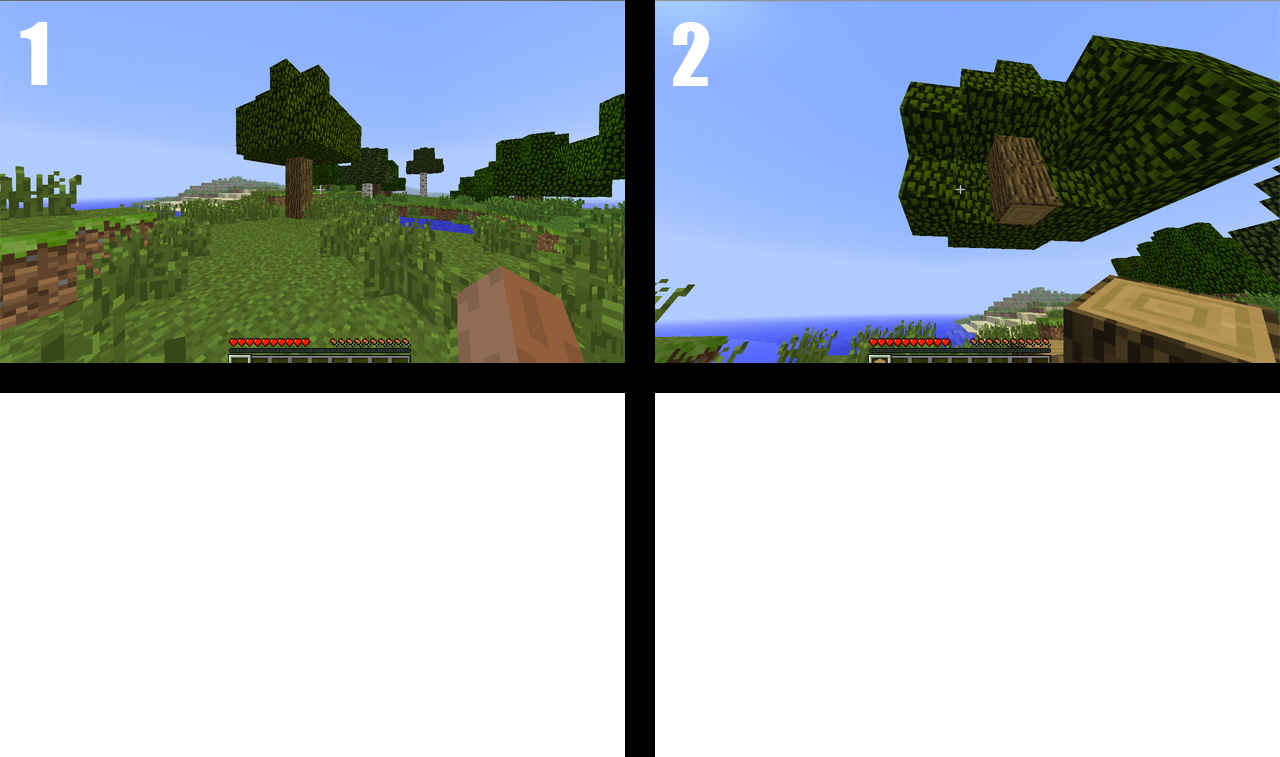
\includegraphics[width=15cm]{graphics/minecraft_mechanics}
  \caption{Minecraft Basic Mechanics  (CC-BY-3.0 Mojang AB)} %TODO find out copyright
  \label{mc_mechanics}
\end{figure}

        \subsection{The Client Server Protocol}
Minecraft's Client-Server-Protocol is not publicly documented by the developers themselves. However, the modding-community gathered full knowledge and understanding of its structure (probably by using reverse engineering techniques). The protocol is based on packets. 

%TODO mention NBT file format

Packets are either "server to client", "client to server" or "two-way" and begin with a "Packet ID" byte. The structure of the packet's payload depends on it's Packet ID.
 
To give an example of one of the easier packets, the "Client Position"-Packet is fairly straight-forward~(see figure \ref{mc_packet}). It is exclusively send from clients to servers and starts with it's Packet ID (as every packet does), followed by the X- and Y-coordinates as doubles, the stance value as a double, which is used to modify the player's bounding box, another double for the Z-coordinate and eventually a boolean that describes if the player is on the ground or not.~\cite{protocol}

\begin{table}[htb]
\centering
\begin{tabular}{|c|c|c|}\hline

    Field Name & Field Type & Notes \\ \hline
   Packet ID & Byte & 0x0B \\ \hline
   X & double & Absolute position \\ \hline
   Y & double & Absolute position \\ \hline
   Stance & double & Used to modify the players bounding box \\ \hline
   Z & double & Absolute position \\ \hline
   On Ground & boolean & Derived from packet 0x0A \\ \hline
   
\end{tabular}
\caption{Structure of the packet ``Player Position (0x0B)''~\cite{protocol}}
\label{mc_packet}
\end{table}

Knowledge of this data structure is already sufficient to move around in the Minecraft world. To go forward, one has to figure out the players current position, calculate the absolute coordinates of the destination of the movement in regard of it and send a Client Position packet with these coordinates via a TCP socket to the server. If the destination is not more than 100 blocks away from the origin of the movement, the server accepts the movement. In the official Minecraft client, a player's movement from one point to the other is rendered with a walking animation.

Other than movement, packet structures are defined for every aspect of the game. May it be the initial handshake, the creation or destruction of blocks or activities of other player- or non-player-characters.

This protocol is what a custom Minecraft client needs to speak.

    \section{Minecraft as a Gaming Platform}
With more and more applications that move beyond the original construction and survival, Minecraft seems to slowly shift towards being not only a game, but a gaming platform, that many other people use to implement their own ideas. Inside Minecraft worlds players build games for educational purposes. A group of students of the Miami University developed a game called Circuit Magic that is dedicated to teach the player about Logical circuits. The infamous Minecraft Teacher, who implements Minecraft in primary school classes, is another good example. Following in his footsteps, ``Massively Minecraft'' is a community of teachers who share their thoughts and experiences with doing the same. Just as well, games have been developed for the purpose of artistic expression. Chain World, the game that tried to simulate religion, is an interesting bit. Not only do players implement their engagement inside Minecraft. The internet is full of Minecraft content, be it videos on youtube, online tutorials or community based knowledge resources, head-quartered at the Minecraft Wiki ( http://www.minecraftwiki.net/ ) .~\cite{Duncan:2011:MBC:2207096.2207097}

As user-generated content has been an essential part in the development of Minecraft, in a process that reminds one of a self-fulfilling prophecy, more and more people explore its possibilities to experiment with new applications. As of today, Persson and Mojang seem to favour and approve new uses of their creation.~\cite{Duncan:2011:MBC:2207096.2207097}

    \section{Suitability of Minecraft as a Simulation Environment}
There are a number of reasons why using Minecraft as a simulation environment could be useful and lead to interesting results.

First, the game itself is easily accessible. It is developed using Java (for both the client and the server software) and therefore, up to a certain extend, platform independent. The "desktop computer version" is being sold for Windows, Mac OS X and Linux devices. There are official ports for Android, iOS, Xbox 360, the Raspberry Pi and a version for the upcoming gaming console Xbox One is announced. The desktop versions are priced at 19.95 euros, which makes it affordable to a large audience.
%TODO find out how to typeset €

The game itself already has an enormous fanbase. It is (like most videogames) especially popular among teenagers. Minecraft being loved by so many people could benefit this project, in terms of leading to increased attention.

The game's developer has proven many times that it acts generously towards  other developers, when it comes to the creation of game modifications and content that uses or changes original Minecraft intellectual property. In other words: Mojang is not restrictive towards users doing all kinds of things with their creations. This led to the availability of a fairly complete community-sourced  documentation and explanation of virtually every aspect of the game---including it's software architecture, data structures and protocols. This is useful for this project, as chances are low that they will have anything against using Minecraft for AI simulations in the foreseeable future. %(In fact, the game's A.I. creator Jon Kagström seems to be fond of this project)

The Minecraft world with it's logic, semantic and functionalities offers possibilities for an AI to prove being able to interact with the environment---in primitive ways (e.g. moving around), as well as with increasingly complex tasks like building, collecting resources, crafting items and interacting appropriately with both well-disposed and hostile other entities.

The semantics of the gameworld share characteristics with the real world. Moving through a Minecraft environment, one quickly realises that the game has generated different biomes (eg. forest or tundra). Also, trees, rivers, mountains and ore veins are neither hard-coded, nor appear completely randomly, but are generated procedurally and their structure appears to be (somewhat) fractal.
        
Using Minecraft as a simulation environment will give Psi agents possibilities to show off, what kind of sophisticated behaviour they are capable of.

    \section{Related Projects}
Minecraft's success inspired many other projects, including artificial players and a number of Minecraft-like games in a wide variety of programming languages and environments.


        \subsection{Minecraft Bots}
There exist many projects, that could be considered Minecraft ``bots''. One has to differentiate in between two types. On the one hand there are those, that mimic an entire client software and facilitate communication with the server on the default client software's behalf. On the other hand, there are bots which are modifications of the original client (or server) software and usually add non player characters---like animals and other non-human creatures---to the game. The code is usually injected through one of the popular ``modloaders'' (eg. Minecraft Forge).

One example (and probably the most advanced one), for an entire bot framework that replaces the client, is Mineflayer~\cite{github_mineflayer}. It has a high-level abstraction of the environment (eg. entity knowledge and tracking) and is written in JavaScript using node.js. However, it has not been used for this project, because a Python implementation was aimed for.

Opposed to Mineflayer, an example for ``game modification'' bots are the ``Cubebots''---fan-made non-player characters that aim to help Minecraft players with mundane tasks~\cite{mcforums_cubebot}.

    \subsubsection{\texttt{Spock} by Nick Gamberini}
Developed by Nick Gamberini, \texttt{Spock} is an open-source bot framework (and as such also a Minecraft client) written in Python. It has been chosen to become an essential part of this project for two reasons: being written in Python it painlessly integrates in the existing MicroPsi code and the absence of dependencies (with one exception) leave the code understandable and easy to deploy. %TODO what exception?
    
    \subsubsection{Protocol Implementation in \texttt{Spock}}
The Minecraft protocol implementation in \texttt{Spock} is straight-forward~(see listing~\ref{snippet_structures}). The necessary data structures are stored separately and can be accessed globally.

		
		\begin{figure}[ht]
			\centering
			\begin{minipage}{11cm}
				\begin{pseudocode}
names = {
	0x00: "Keep Alive",
	0x01: "Login Request",
	0x02: "Handshake",
	0x03: "Chat Message",
	...

structs = {
	#Keep-alive
	0x00: ("int", "value"),
	#Login request
	0x01: (
			("int", "entity_id"),
			("string", "level_type"),
			("byte", "game_mode"),
			("byte", "dimension"),
			("byte", "difficulty"),
			("byte", "not_used"),
			("ubyte", "max_players")),
	...
					\end{pseudocode}
				\caption{data structures for the packet IDs and structures}
				\label{snippet_structures}
			\end{minipage}
		\end{figure}
		
These structures are used to parse each packet appropriately~(see listing \ref{snippet_parse}).

		\begin{figure}[ht]
			\centering
			\begin{minipage}{13cm}
				\begin{pseudocode}
	def decode(self, bbuff):
		#Ident
		self.ident = datautils.unpack(bbuff, 'ubyte')
		
		#Payload
		for dtype, name in mcdata.structs[self.ident][self.direction]:
			self.data[name] = datautils.unpack(bbuff, dtype)
					\end{pseudocode}
				\caption{function for decoding packets}
				\label{snippet_parse}
			\end{minipage}
		\end{figure}
		
		\subsection{Minecraft Clones}
Other interesting projects include Skycraft~\cite{skycraft}, a Minecraft-like browser-game based on WebGL.

A particular project, that has the same name as the original game that inspired it, is \texttt{Minecraft} by Michael Fogleman~(see figure~\ref{fogleman_mc_screen}). It is a simple Minecraft clone in under 600 lines of Python and gained some popularity on reddit~\cite{fogle-reddit} and Hacker News~\cite{fogle_hn}.

It is comparably easy to understand and modify and has been used for the visualisation component of this project. It is based on the Python multimedia library Pyglet~\cite{pyglet}.

\begin{figure}[h]
  \centering
    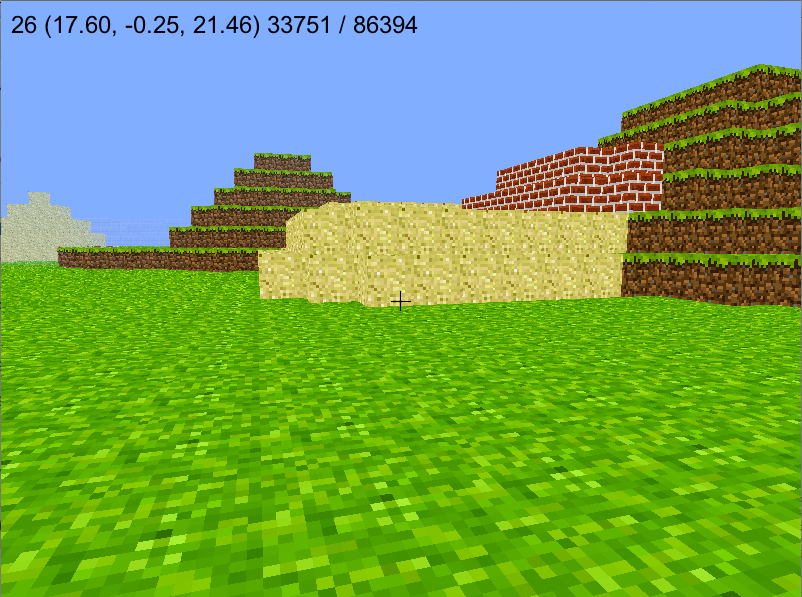
\includegraphics[width=10cm]{graphics/fogleman_mc_screen}
  \caption{\texttt{Minecraft} by Michael Fogleman}
  \label{fogleman_mc_screen}
\end{figure}

    \section{Summary}
Minecraft is a complex, yet easily accessible virtual world. It is in constant development and new features are added regularly. It has a massive fanbase and a huge community around all kinds of game-modifications.